\documentclass[12pt,titlepage]{scrreprt}
\usepackage[ngerman]{babel}
\usepackage[utf8]{inputenc}
\usepackage{color}
\usepackage{float}
\usepackage[a4paper,lmargin={2.5cm},rmargin={2.5cm},tmargin={2.5cm},bmargin = {2cm}]{geometry}
\usepackage{amssymb}
\usepackage{amsthm}
\usepackage{graphicx}
\usepackage{subfig}
\usepackage{wrapfig}
\usepackage{url}
\usepackage{cite}


\begin{document}
% % Activate the following line by filling in the right side. If for example the name of the root file is Main.tex, write
% "...root = Main.tex" if the chapter file is in the same directory, and "...root = ../Main.tex" if the chapter is in a subdirectory.
 
%!TEX root =  TNTinderSee.tex

% mehrere Bilder in einer Bildumgebung mit 
%\subfloat{bild.jpg}


\begin{titlepage}
\thispagestyle{empty}
 \begin{center}
 \begin{figure}[htbp]
    \centering
 %   \subfloat{\includegraphics[width=0.15\textwidth]{Bilder/Titel/bild-firma.JPG}}\quad
   %  \subfloat{\includegraphics[width=0.25\textwidth]{Bilder/Titel/bild-uni 
%oder fh.JPG}}
\end{figure}
\vspace*{1cm}
 \Large{Schiller-Gymnasium Offenburg }

  \vspace*{1.5cm}
 {\huge Thema}
 \vspace*{1cm} \\
 {\Large Abschlussbereicht\\von\\Eitel, Martin \\ \texttt{marjelly1@gmail.com}\\Komyakov, Alexander \\\texttt{alexander.komyakov@lynxisgod.eu} \\ Rehwinkel, Antonio \\ \texttt{antonio.rehwinkel@schiller-og.de} \\ Sauerbrey, Luisa \\ \texttt{luisa.sauerbrey@schiller-og.de}
 \vspace{0.5cm}
 {\Large \bfseries \\}
 \vspace{0.5cm}
 {\Large geboren am dein Geburtstag}
 \vfill
  \vspace*{1.5cm}
\begin{table}[h]
	\centering
	\begin{tabular}{|l| l|}\hline
		Aufgabensteller & Prof. \\ \hline
		Durchgeführt bei: & Firmenname\\ \hline
		Betreuer: & Betreuer Firma\\ Marek Czernohous \\ \hline
		Wissenschaftspate & \\ Prof. Dr. Jens Greinert\\ \hline
		Arbeit vorgelegt am: & Datum\\ \hline
	\end{tabular}
\end{table}
}
\end{center}
\end{titlepage}


\begin{titlepage}

	

\title{Die Auswirkung von Munitionshalden auf die Wasserqualität der Ostsee zwischen Vilm und Lauterbach}
\subtitle{Ausfahrt vom 18.07. - 21.07.2021}
\titlehead{\centering\includegraphics[width=15cm]{Bilder/DSC05220}}


\author{Eitel, Martin; Komyakov, Alexander; \\ Rehwinkel, Antonio; Sauerbrey, Luisa\\ \and Schiller-Gymnasium Offenburg}

\publishers{Wissenschaftspate: Prof Dr. Jens Greinert \texttt{jgreinert@geomar.de} \\
\vspace*{2ex} Betreuer: Marek Czernohous \texttt{m.czernohous@schiller-offenburg.de}}
%- \\ Schiller-Gymnasium Offenburg}

\maketitle

\end{titlepage}
\addchap{Kurzfassung}
Unser Wettbewerbsbeitrag umfasst

\tableofcontents
% Activate the following line by filling in the right side. If for example the name of the root file is Main.tex, write
% "...root = Main.tex" if the chapter file is in the same directory, and "...root = ../Main.tex" if the chapter is in a subdirectory.
 
%!TEX root =  TNTinderSee.tex

\chapter[Einleitung]{Einleitung}

Im Meer lagernde Munition stellt eine Gefahr dar. Nicht unbedingt durch unmittelbare Detonotationsgefahr, 
sondern durch die langsame Zersetzung, die die enthaltenen Sprengstoffe nach und nach 
freilegt\cite{zeitbomben}. Die Entstehung sprengstofftypischer Abbauprodukte, sowie das direkte Austreten 
giftiger Stoffe, stellen Gesundheitsgefährung exponierter Meerestiere, aber auch Menschen dar, denn die
Abbauprodukte gelten als krebserregend und das potentiell austretende Phosphor lagert sich an den Stränden 
ab und ist von Bernstein kaum zu unterscheiden. Als wir den Meereswettbewerb mit der Aldebaran fanden, 
fühlten wir uns gezwungen nachzuforschen wie groß die Gefahr schon heutzutage ist.\\

Wir wollten in einem potentiellem Munitionsabwurfsgebiet messen, wie groß die Anteile der Schadstoffe sind und 
ob noch etwas von den Granaten und Bomben zu sehen ist. Dazu entschieden wir uns für ein Gebiet kurz Vilm,
da hier angeblich zwei Schuten nach dem Zweiten Weltkrieg mit Munition beladen explodiert sein sollen.\\

Das Naturschutzgebiet Vilm liegt in etwa 100 Meter Entfernung zu der Explosionsstelle und auch weiter 
entfernte Orte können durch Ablagerungen und Schadstoffe in Fisch-Fängen betroffen sein.\\

In Zusammenarbeit mit der Aldebaran und dem Geomar wollten wir die Wracks kartieren und die Schadstoffwerte in
der direkten Umgebung messen. Besonders interessant wäre die beförderte Munition gewesen. Die Frage der
Ortung und Untersuchung der möglichen Funde konnten wir zusammen mit dem Geomar lösen. Mithilfe eines 
"Multibeams" sollten wir interessante Orte ohne Tauchgang finden können um später mit dem Schuleigenen 
ROV die Orte genauer unter die Lupe nehmen zu können. Auch Sedimentproben dirket neben den Fundstätten 
konnten wir mithilfe eines eignene Aufsatzes realisieren.\\

Wir befürchteten hohe Werte für Phosphor und sprengstofftypische Verbindungen wie Trinitrotoluol (TNT) 
zu messen und unter Umständen sogar Granaten oder Bomben zu finden. Falls dies passieren sollte, würde 
sich für uns die Frage stellen, wie sich diese Munition auf die Öknomie ausgewirkt hat. \\

In schon existierenden Forschungen zeigt sich, 
https://www.schleswig-holstein.de/DE/UXO/EN/Themes/Subjects/assessements.html

https://www.geomar.de/fileadmin/content/service/presse/Pressemitteilungen/2020/pm_2020_37_munition-sh.pdf

https://www.eskp.de/schadstoffe/wie-weiter-mit-den-kampfmittelaltlasten-im-meer-9351103/

https://www.eskp.de/schadstoffe/wie-weiter-mit-den-kampfmittelaltlasten-im-meer-9351103/

Themenfindung, Relevanz, entscheidende Fragen, Lösungsansätze, Forschungsstand mit Quellen, Erwartungen, konkrete Fragen.

\chapter{Hauptteil}
\section{Versuchsplanung}
Alle Kartierungsvorgänge wurden mit der Free Open Source Software\\
\emph{QGIS}\cite{qgis}durchgeführt.
\begin{figure}[ht]
    \centering
    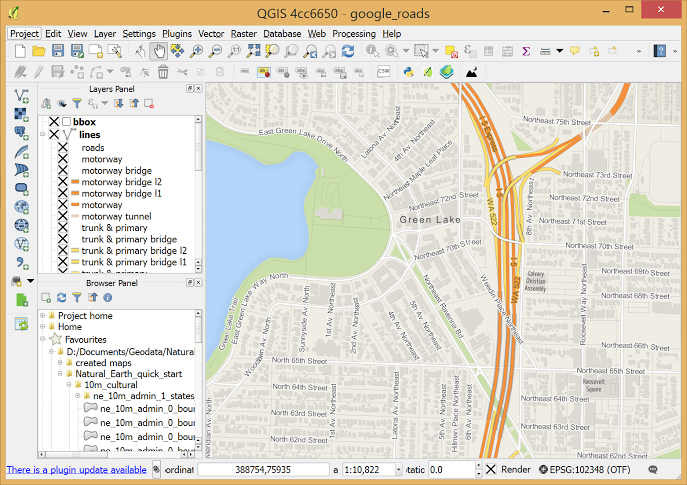
\includegraphics[width=.4\linewidth]{Bilder/QGIS/about-screenshot.png}
    \caption[fig:qgisabout]{QGIS-Benutzeroberfläche}
\end{figure}
\\Mithilfe dieser Software lassen sich basierend auf bereits existierenden Karten, 
wie beispielsweise \emph{OpenStreetMap}\cite{ostrm} oder \emph{OpenSeaMap}\cite{oseam},
eigene Routen und Points of \\Interest(POIs) ohne großen Aufwand eintragen. Genauso 
leicht erfolgt der Import sowie vom Multibeam,  als auch von den Navigationsgeräten 
der ALDEBARAN gespeicherten Positions- und Geschwindigkeitsdaten.\\


Basierend auf dem QGIS-Projekt von \jens, welches die \emph{OpenStreetMap}, sowie den Munitionslagerstättendaten von den Webseiten
\emph{AmuCad}\cite{amucad} und \emph{Munition im Meer}\cite{muninmeer}
als Basis benutzt, konnten wir unsere Route planen (vgl. Abbildungen \ref{fig:route} und \ref{fig:multibeam_route}).

\begin{figure}[]
    \centering
    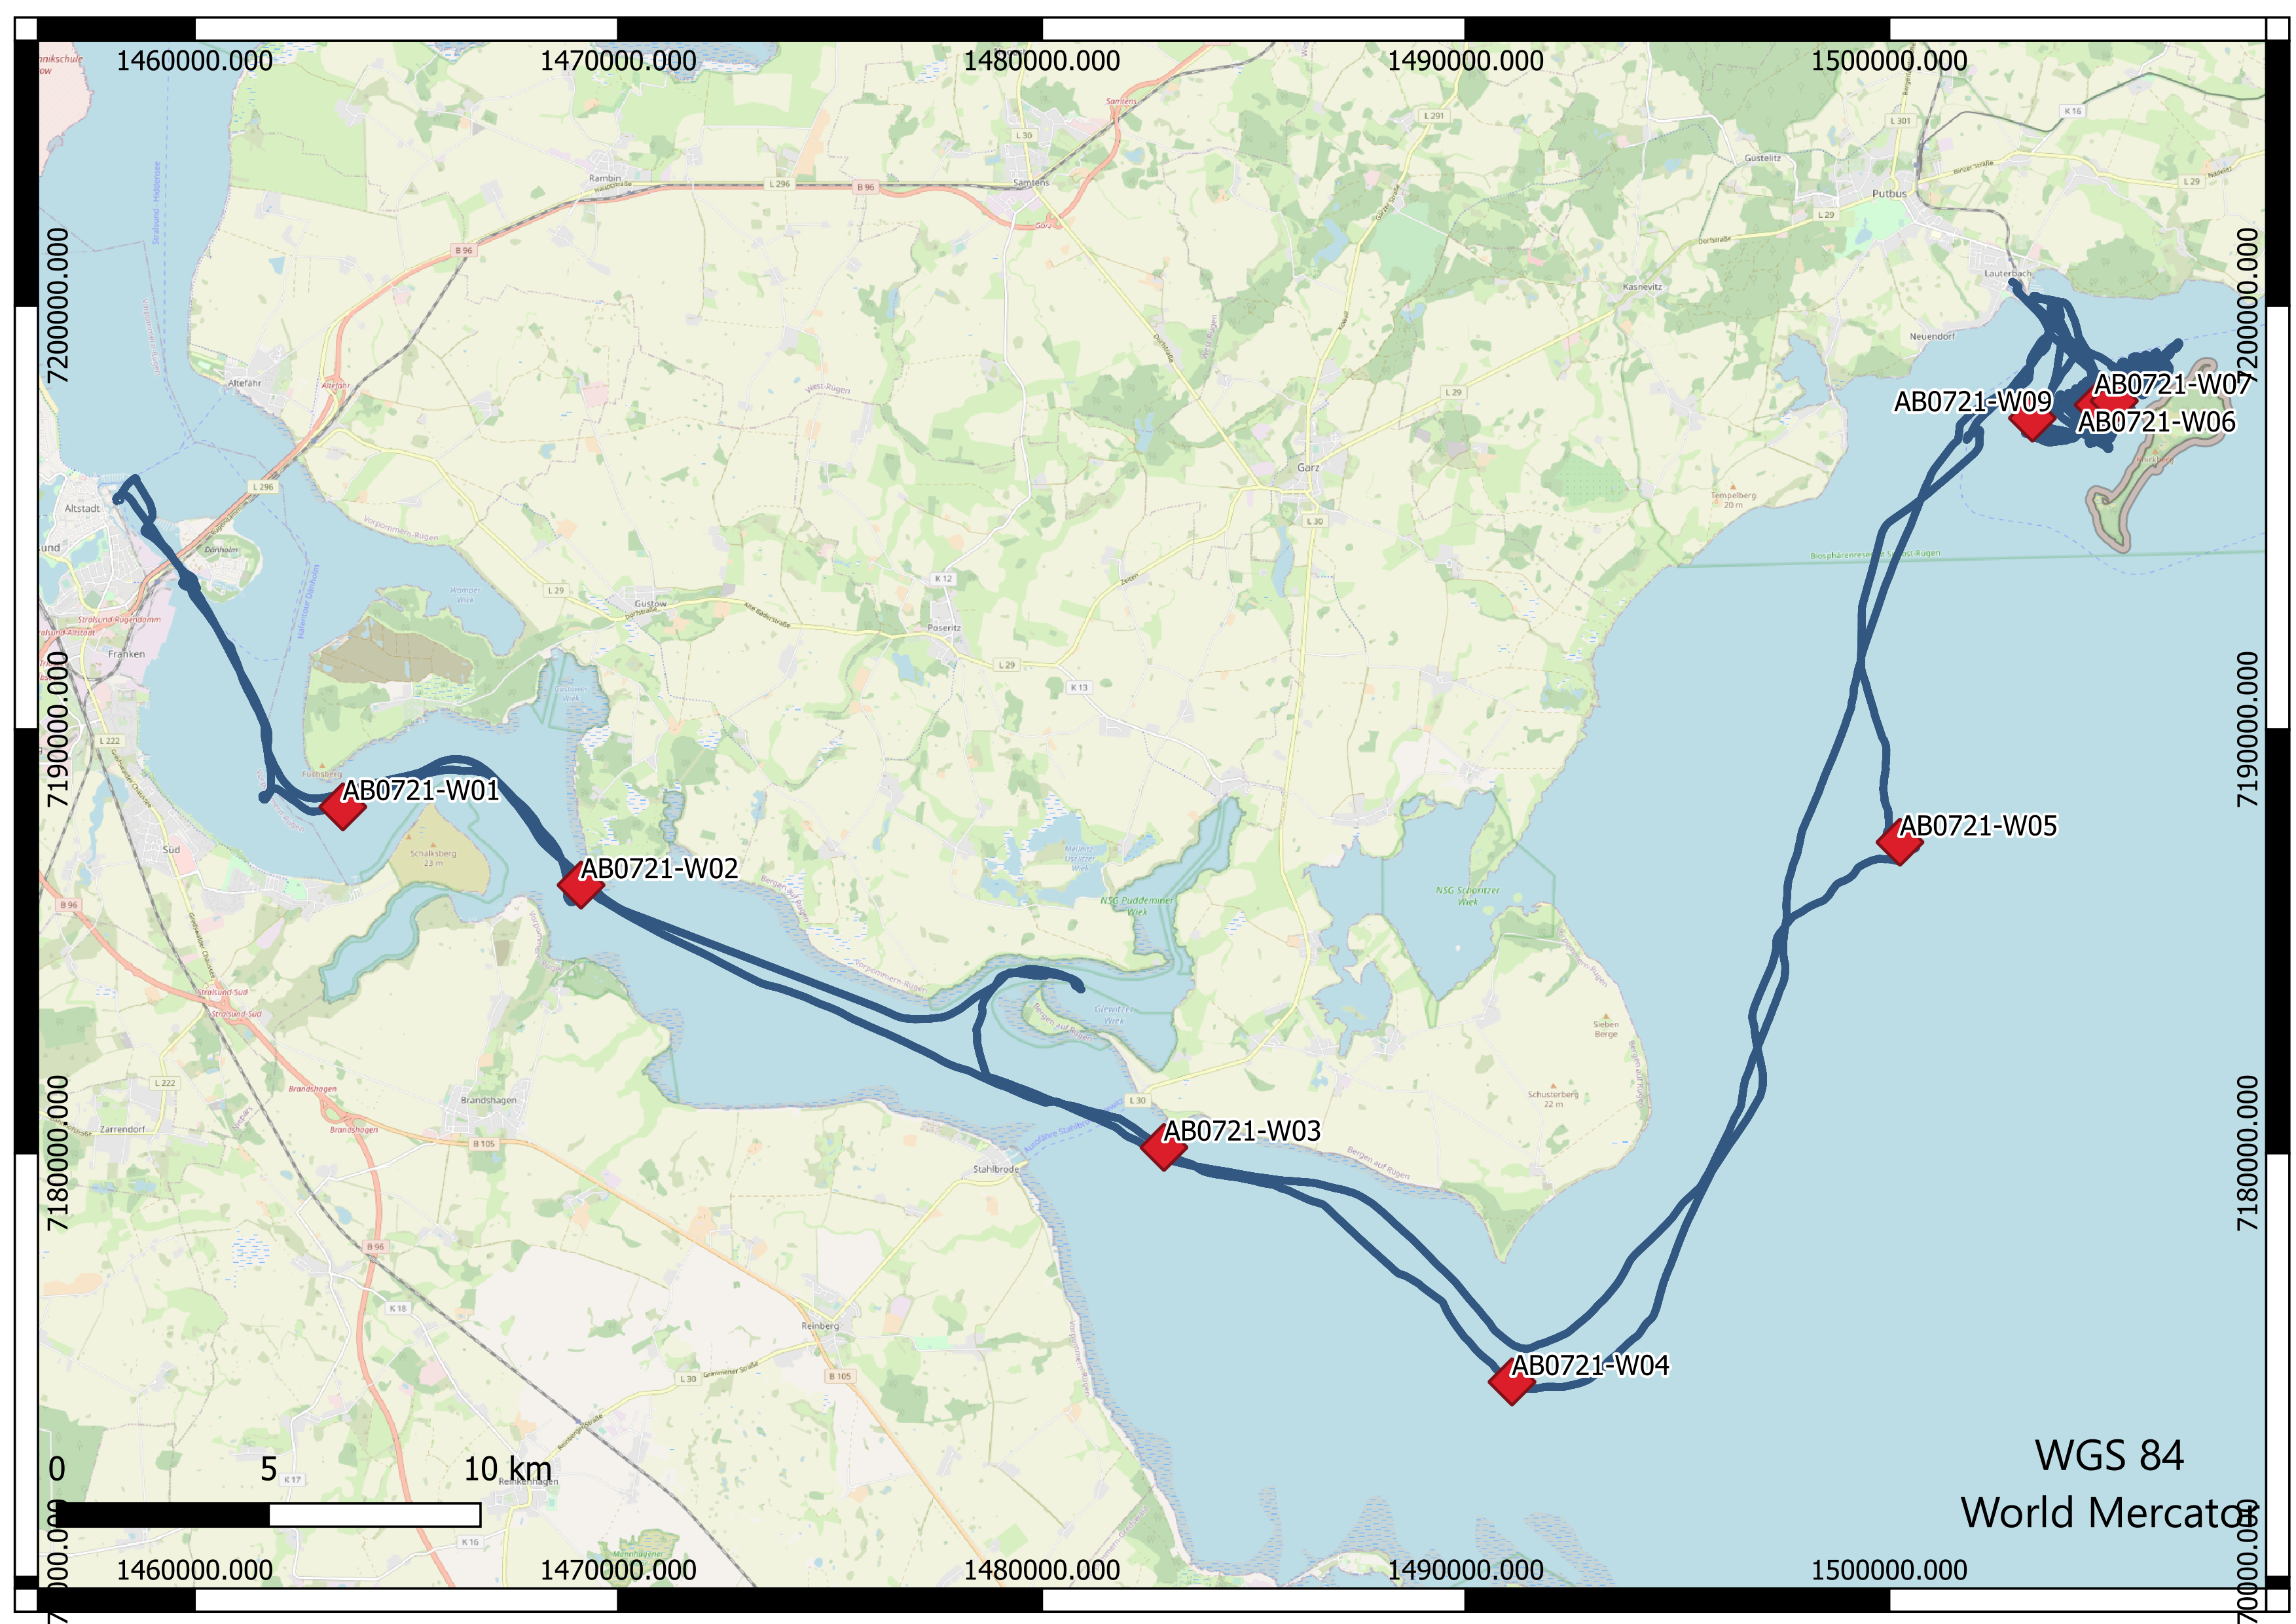
\includegraphics[width=0.8\linewidth]{Bilder/QGIS/Gesamte_route.png}
    \caption{Gesamte Route}
    \label{fig:route}
\end{figure}
\begin{figure}[]
    \centering
    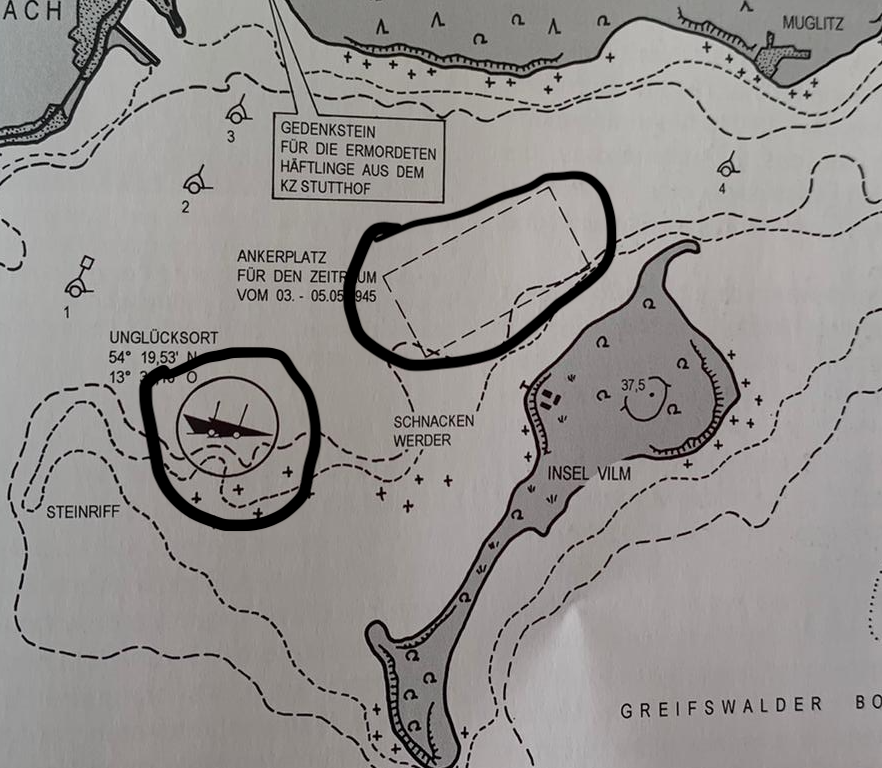
\includegraphics[width=0.8\linewidth]{Bilder/ungl.png}
    \caption{Dokumentierte Anker und Unglückstelle der Sprengstoffschuten.\cite{schiffsschicksale}}
    \label{fig:unglueck}
\end{figure}
\begin{figure}
    \centering
    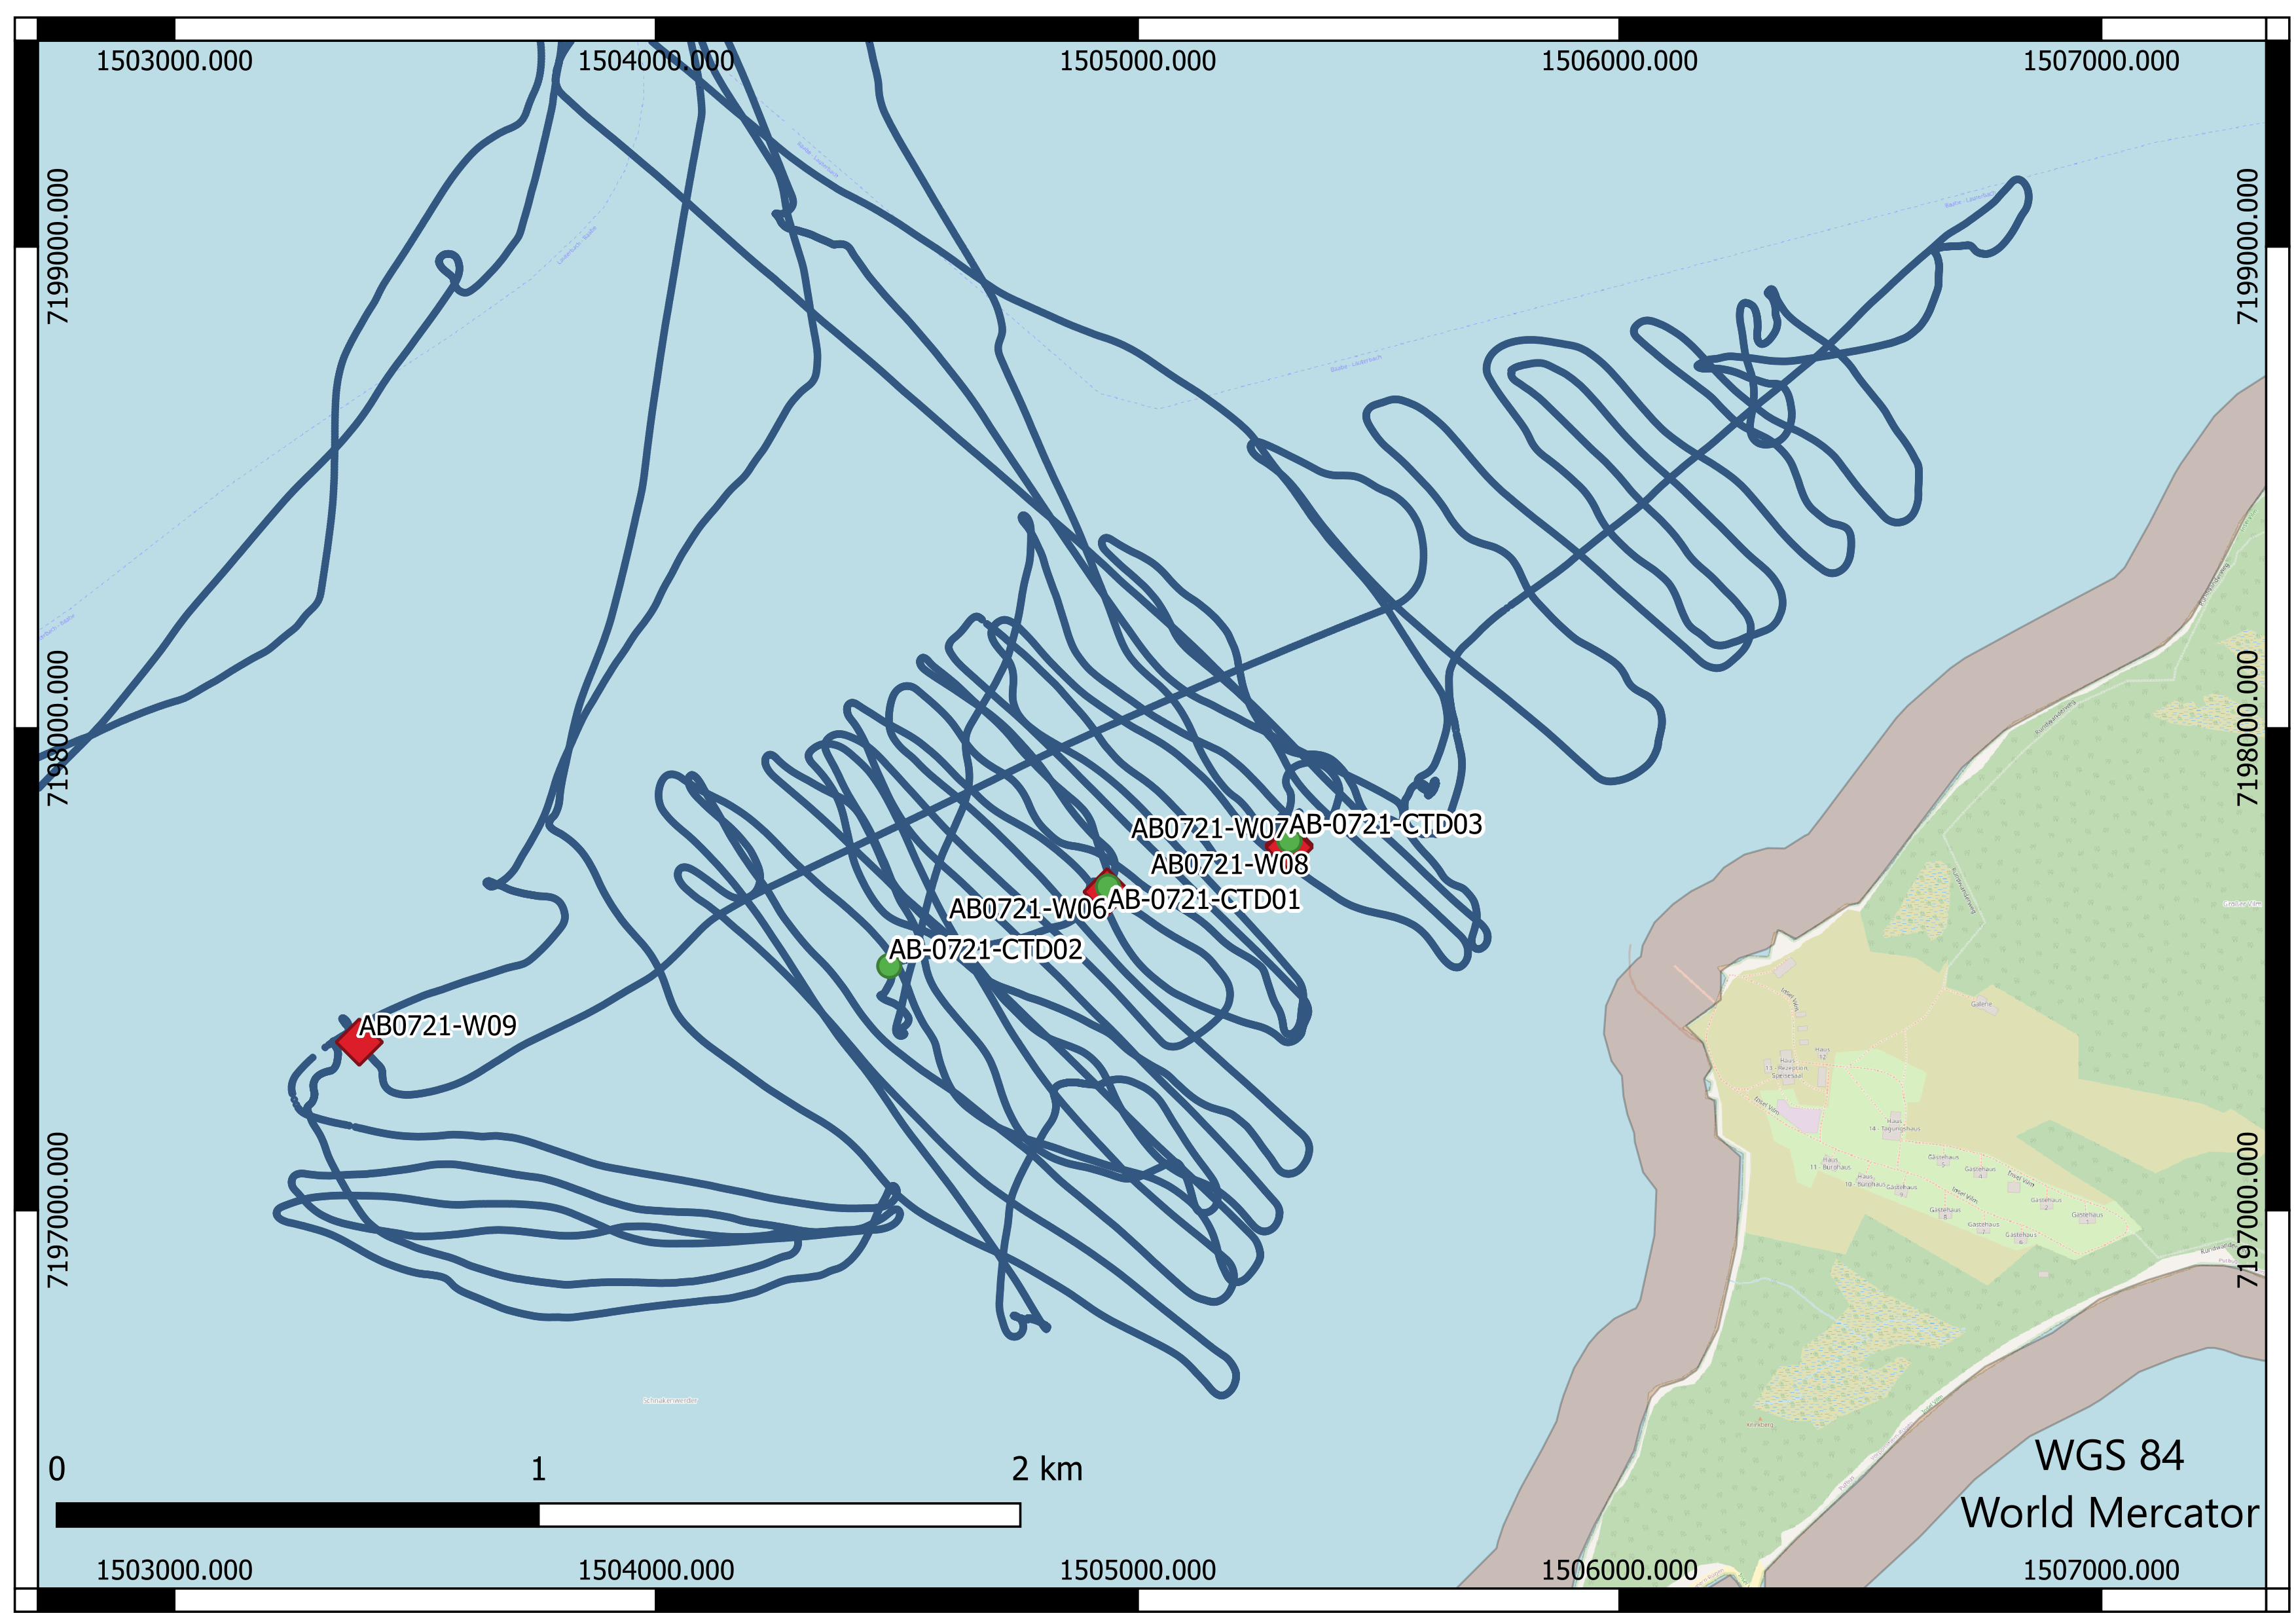
\includegraphics[width=0.8\linewidth]{Bilder/QGIS/multibeam.png}
    \caption{Multibeamfahrten. Wasserproben- und CTD-Stellen sind\\jeweils rot und grün markiert.}
    \label{fig:multibeam_route}
\end{figure}

%% Activate the following line by filling in the right side. If for example the name of the root file is Main.tex, write
% "...root = Main.tex" if the chapter file is in the same directory, and "...root = ../Main.tex" if the chapter is in a subdirectory.
 
%!TEX root =  TNTinderSee.tex

Um den sprengstofftypischen Verbindung auf die Spur zu kommen, war es unabdinglich, an verschiedenen Orten Wasserproben zu nehmen. Die Probe muss dabei nicht etwa in unmittelbarer Nähe von Minen, Bomben o.ä. genommen werden, da sprengstofftypische Verbindungen typischerweise auch noch an weiter entfernten Positionen nachzuweisen sind. Wir entschieden uns für Probenaufnahmen in der Nähe des ehemaligen Ankerplatzes und des Unglücksortes der 1945 gesunkenen Schute.

\subsubsection{Technische Beschreibung und Durchführung an Board}
Die Wasserbeprobung ist relativ simpel. Wir hatten dafür ein Plastikrohr mit Deckeln, welche mithilfe von zwei Gummis offen gehalten wurden. Das Rohr wurde ins Wasser gelassen, jeweils abgestimmt auf die Wassertiefe Tiefe abzüglich eines Meters, so dass aufgewirbelter Dreck oder Algen nicht im Weg waren. Sobald sich das Plastikrohr an der richtigen Stelle befand, wurde ein kleines metallenes \emph{Engelchen} dem Seil entlang, an welchem das Rohr befestigt war, in die Tiefe geschickt. Das Engelchen war aufgrund von seinem Material relativ schwer, wodurch sich die Gummis an dem Rohr lösten und die Deckel zu gingen. Danach musste die Probe nur noch hoch gezogen werden.

Sobald sich die Probe wieder auf dem Boot befand, konnten wir weiter zum nächsten Standpunkt fahren. Auf dem Boot ging dann allerdings erst die richtige Arbeit los, nämlich aus der rohen Wasserprobe eine zu machen, aus welcher man auch Informationen ziehen konnte. An dem Rohr befand sich ein kleines Ventil, wodurch wir das Wasser langsam und kontrolliert in einen Messbecher laufen lassen konnten. Mit viel Feingefühl versuchten wir genau 1000ml zu bekommen. Es würde keinen großen Unterschied machen, wenn es mehr oder weniger wäre, allerdings hat uns das Abmessen einiges an Rechnen erspart. 

Das abgemessene Wasser wurde anschliessend durch einen selbst gebauten Trichter in ein \emph{Blood Bag} gefüllt, solche wie man auch bspsw. bei Operationen im Krankenhaus findet, um Blut zu lagern. In unserem Fall war dies allerdings nur ein Zwischenschritt. 
An dem Blood Bag befestigten wir einen kleinen Schlauch mit einem Filter, durch dass das Wasser gelassen wurde. Im Anschluss an den Filter, welcher lediglich Schmutzpartikel aus dem Wasser filterte, befand sich ein kleines Teströhrchen mit einer Art Granulat. Dieses war nach unten hin offen, da das fertig durchgelaufene Wasser unbrauchbar für uns war, weshalb wir es einfach langsam abtropfen lassen konnten.

Die eigentliche Magie war nun das Geschehen in dem Granulat. Dieses dient dazu, schadstoffähnliche Verbindungen aus dem Wasser zu filtern und zu speichern. 

\subsubsection{Probenpräparation am GEOMAR}
Die Teströhrchen haben wir anschließend mit ins Geomar nach Kiel genommen. Dort haben wir die Proben für den Ionenchromatographen präpariert, indem wir eine definierte Menge von destilliertem Wasser über das Granulat haben laufen lassen. Anschließend wurden die Proben mit einem Verdünnungsmittel auf 2ml aufgefüllt. Diese nun fertige Probe wurde dann auf Rückstände sprengstofftypischer Verbindungen analysiert.
\begin{figure}[]
    \centering
    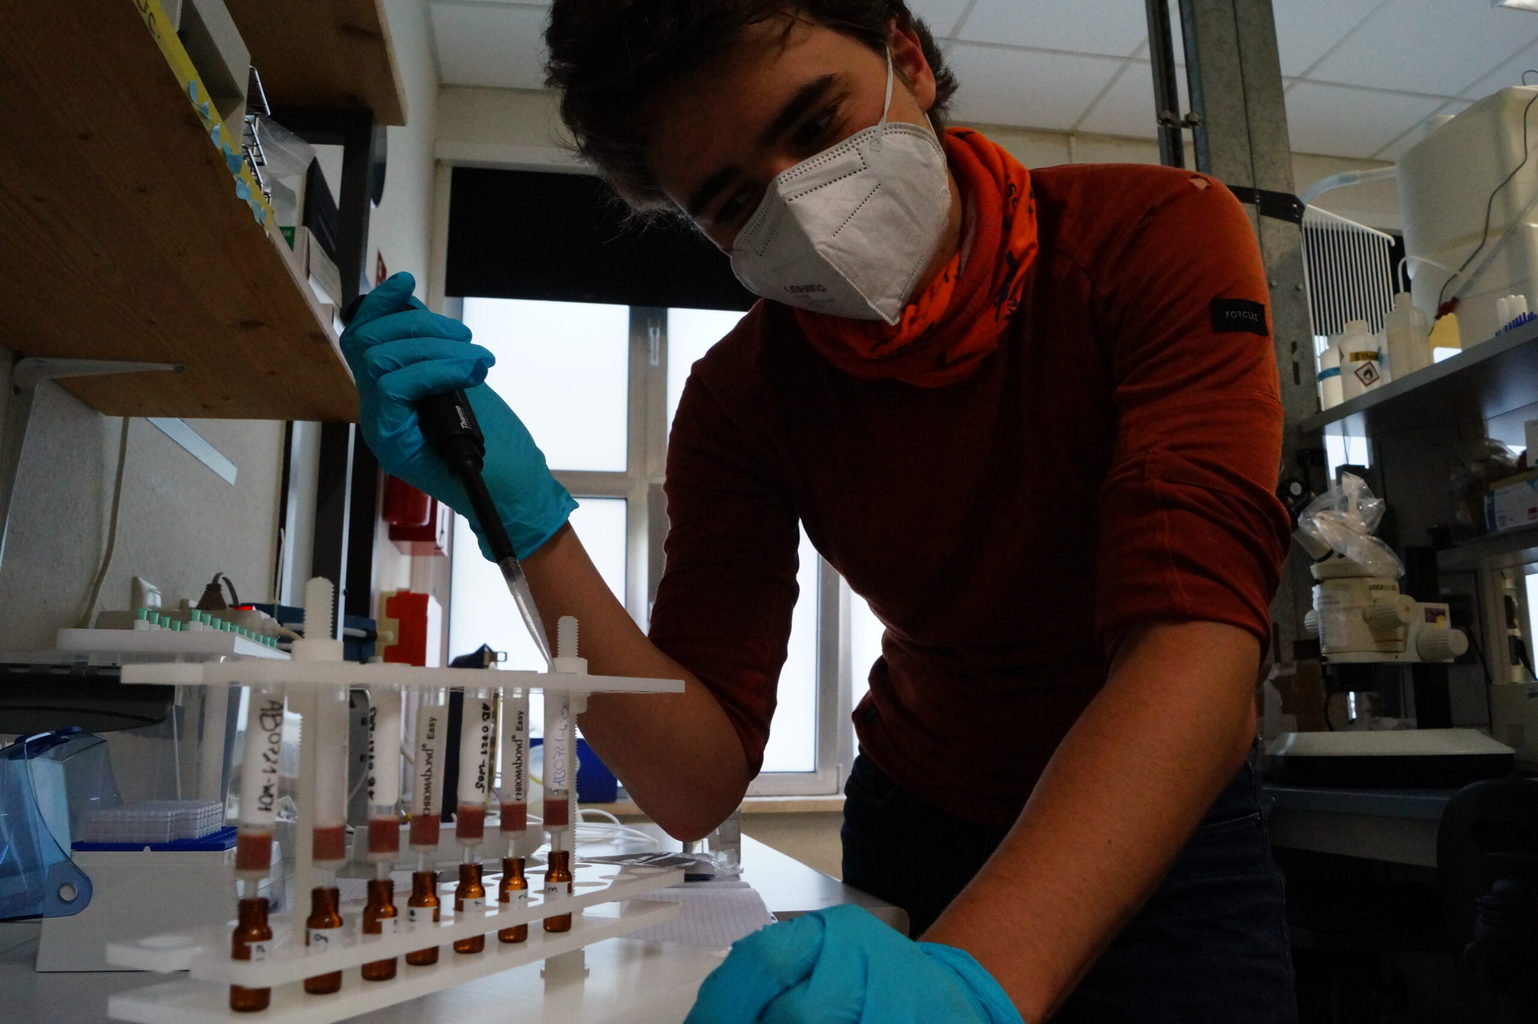
\includegraphics[width=0.8\linewidth]{Bilder/DSC05766-scaled.jpg}
    \caption{Vorbereitung der Wasserproben für den Ionenaustauschchromatographen}
    \label{fig:praep}
\end{figure}
\subsection{Multibeamparametermessungen}
% Activate the following line by filling in the right side. If for example the name of the root file is Main.tex, write
% "...root = Main.tex" if the chapter file is in the same directory, and "...root = ../Main.tex" if the chapter is in a subdirectory.
 
%!TEX root =  TNTinderSee.tex

Da das vollständige Abfahren des Gebiets mithilfe des ROVs zeitlich und stromtechnisch nicht 
möglich gewesen wäre, brachten die Forscher des Geomar ein Multibeam mit auf die Aldebaran. \\

Ein Multibeam funktioniert ähnlich wie ein Echolot, es sendet eine Schallwelle in die zu messende 
Richtung und wartet darauf dieses Signal wieder zurückzubekommen. Durch den Zeitunterschied 
kann die Entfernung bestimmt werden. Der größte Unterschied zwischen einem Echolot und dem Multibeam 
liegt bei der Anzahl der "Beams". \\

Das von uns verwendete Multibeam kann mit 512 Einzel-Echoloten in einem Winkel von 130° großflächig den
Meeresboden kartieren und dies 
deutlich genauer als unsere ROV-Kamera es schaffen könnte. Da die zu messenden Schallwellen des Multibeams 
sich kegelförmig ausbreiten haben wir auf dem Meeresboden ein Quadrat, dessen Größe die Auflösung unseres Multibeams beschreibt.
Wir stellen die Genauigkeit des Multibeams, später "Grid" gennant, zu Anfang auf 25cm$^2$ um den Computer nicht zu überlasten, aber 
noch immer kleine Gegenstände zu finden.\\

Da die Schallgeschwindigkeit in jedem Gewässer leicht unterschiedlich ist, wurde auf dem Multibeam
ein Schallgeschwindigkeitsmesser montiert. Doch nicht nur hier kann sich die Geschwindigkeit ändern!
Auch innerhalb des Wassers gibt es Schichten, in denen der Schall sich langsamer fortbewegt als in
der Schicht darüber oder darunter. Dadurch kommt es zu Brechungen des "Beams" und der tatsächliche 
Strahlungswinkel des Multibeams verändert sich. Dies hat dann wiederrum einen Effekt auf die finale Kartierung.
Ab einer Tiefe von mehr als 10 Meter muss dieser Effekt beachtet werden. Da unser Forschungsgebiet nur eine 
Tiefe von maximal 7 Meter hat, können wir diesen Effekt vernachlässigen.\\

Jens Greinert und Mareike Kampmeier, beide Mitarbeiter des Geomar, stellen uns das Multibeam zur Verfügung und 
leisten eine großartige Hilfe bei der Kalibrierung und Datenverwertung des selbigen. Die gewonnen Daten werden 
später auch vom Geomar verwendet und analysiert werden. \\

Die Kalibrierung umfasst den Roll, Pitch und Yaw des Schiffes mithilfe eines Bewegungssensors aus den Daten zu 
entfernen und auch die Befestigung des Multibeams am Schiff zu sichern. Da diese Befestigung mobil sein muss, kann
dies nicht so genau wie an einer festinstallierten Stelle passieren. Die Ergebinsse sond dennoch hoch genau. 
Das Multibeam ist mithilfe eines Metallgestells an der Linken Seite der Aldebaran angebracht und kann bei Bedarf 
abgesenkt oder hochgezogen werden.\\

Wir fahren möglichst parallele, gerade Bahnen mit dem Multibeam um eine möglichst hohe Abdeckung zu erreichen. 
Das wir, um die Genauigkeit des Multibeams nicht zu gefährden, nur knapp 3 Knoten schnell fahren dürfen setzt
uns jedoch dem starken Wind aus. \\

Auch die Befestigung des Multibeams ist bringt uns hin und wieder leichte Fehler in die Kartierung. Für die 
Umstände ist das Multibeam trotzdem erstaunlich genau und wir können drei interessante Punkte auf dem 
Meeresboden ausfindig machen. \\
Im Geomar können wir die Rohdaten analysieren. Auch das "Grid", können wir nun verfeinern von 25cm$^2$ auf 10cm$^2$. 
Wir löschen fehlerhafte Daten, erstellen eine 3D-Karte des gescannten Gebiets und erzeugen ein "Backscatter". 
Das "Backscatter" umfasst weniger die Tiefe des Gebiets als die empfangene Laustärke unserer Signale. 
Diese Lautstärke wird von der Tiefe des Gebiets und vor allem von der beschaffenheit des Bodens bestimmt. \\

Generell kann man sagen, das je härter der Boden ist, desto stärker werden die Schallwellen reflektiert. 
Auf der "Backscatter"-Karte wird diese Laustärke veranschaulicht und man kann die Art des Bodens bestimmen.
Auch Munition würde auf dieser Karte stark auffallen, da Sie die Schallwellen starkreflektiert und so 
auf der Karte hell aufleuchten würde. Auf der von uns erzeugten Karte erkennt man die Seegraßwiesen in 
der Nähe der Insel Vilm an ihrer geringen Reflektion

\subsection{ROV-Unterschung}

Unsere grundlegende Idee zur ROV-Analyse war folgende: Erst wollten wir das als munitionsbelastete gekennzeichnete Gebiet mithilfe 
des Multibeams grob kartieren und dabei 
interessante bzw. auffällige Stellen finden. Daraufhin wollten wir diese mit unserem ROV antauchen, um mit unser Kamera eine genauere Bestimmung durchführen zu können. 
Dieses Vorgehen konnten wir auch so zum Großteil durchführen.
Die genauer zu bestimmenden Stellen haben wir mit unserem eigenen ROV (Remotely Operated Vehicle), einer Art Tauchroboter, angetaucht. 
\subsubsection{Technische Beschreibung}
Dieser entstand vor drei Jahren in unsere Forschungsgruppe aus einem Bausatz der Firma BlueRobotics und trägt die Bezeichnung \emph{BlueROV 2}.
Der Tauchrobter lässt sich mithilfe eines Laptops und eines Controllers über ein langes Kabel (auch Tether genannt) frei in alle Richtungen in der Wassersäule bewegen.\\
Das ROV von BlueRobotics besteht aus zwei runden Druckgehäusen eines für den Lithium-Ionen Akku, das andere für die Steuerungselektonik und die Kamera.
Vor jedem Tauchgang müssen diese Druckgehäuse mithilfe einer Vakuumpumpe auf ihre Dichtigkeit überprüft werden. 
\begin{figure}[htb!]
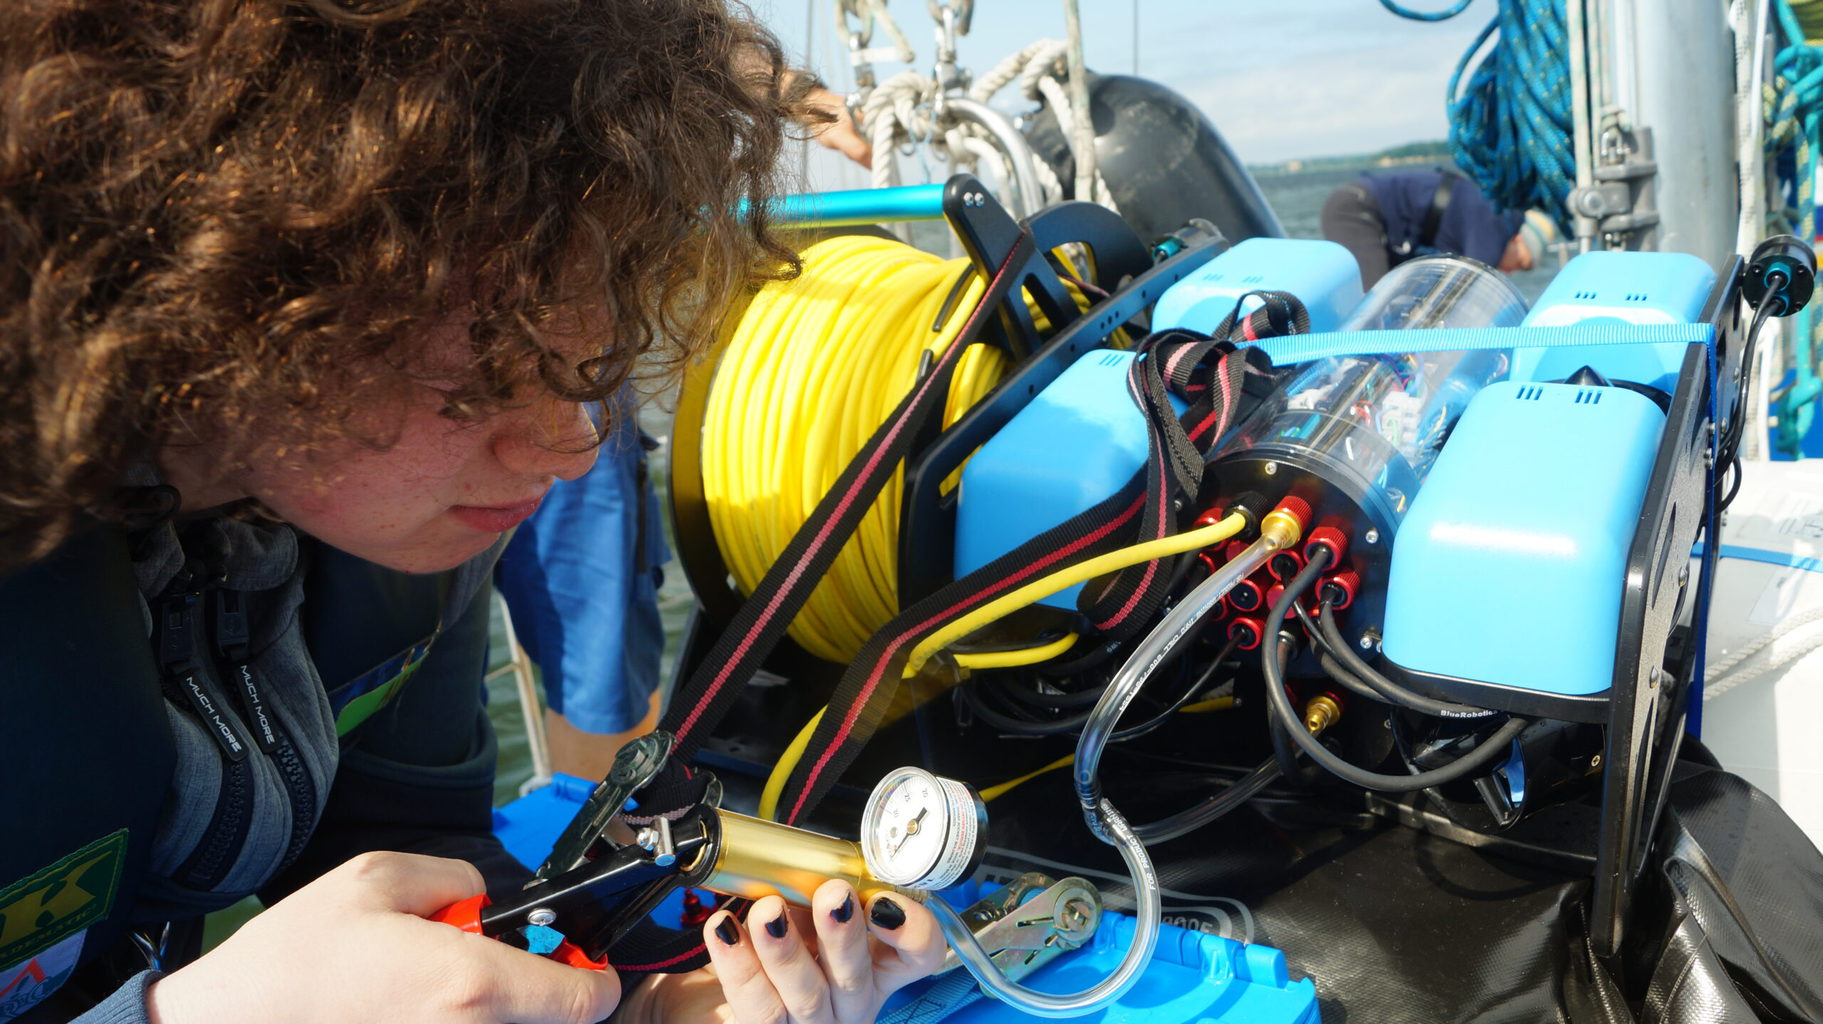
\includegraphics[height=\textheight,%
                   width=\textwidth,%
                   keepaspectratio]{Bilder/ROV/Druckpruefung.jpg}
\caption{Unterdruckprüfung vor der ROV-Fahrt}
\end{figure}
Anschließend wird das ROV mithilfe des Tethers an den Laptop angeschlossen werden, auf dem sich die Steuerungssoftware befindet.
\subsubsection{Operating auf der Aldebaran}
Der ROV wird optimalerweise 
von vier Personen bedient, da zwei Personen die Tetherspule bedienen müssen, man einen Navigator benötigt, da die Orientierung unter Wasser in einem fremdem Gebiet sehr anspruchsvoll ist und das ROV von einem Piloten gesteuert werden muss.
Somit beansprucht das ROV-Fahren unser gesamtes Forschungsteam und kann keine anderen Aufgaben, wie das Positionshalten des Forschungsschiffes o.ä. übernehmen. Deshalb ist das ROV-fahren für die gesamte Crew nicht nur zeitlich durchaus herausfordernd.
Aus diesem Grund war es besonders wichtig, gezielte Stellen ausfindig zu machen, an denen wir mit dem ROV abtauchen wollten und nicht nur blind im Meeresboden rumstochern.
\\

Um die Abläufe des ROV-tauchens richtig einzuspielen und den ROV auf der Aldebaran zu testen, haben wir am Sonntagabend einen Testtauchgang im Hafen durchgeführt. 
Hierbei ist uns schon die schlechte Sicht in der Ostee aufgefallen, die uns später noch einige Schwierigkeiten machen sollte.
\begin{figure}[htb]
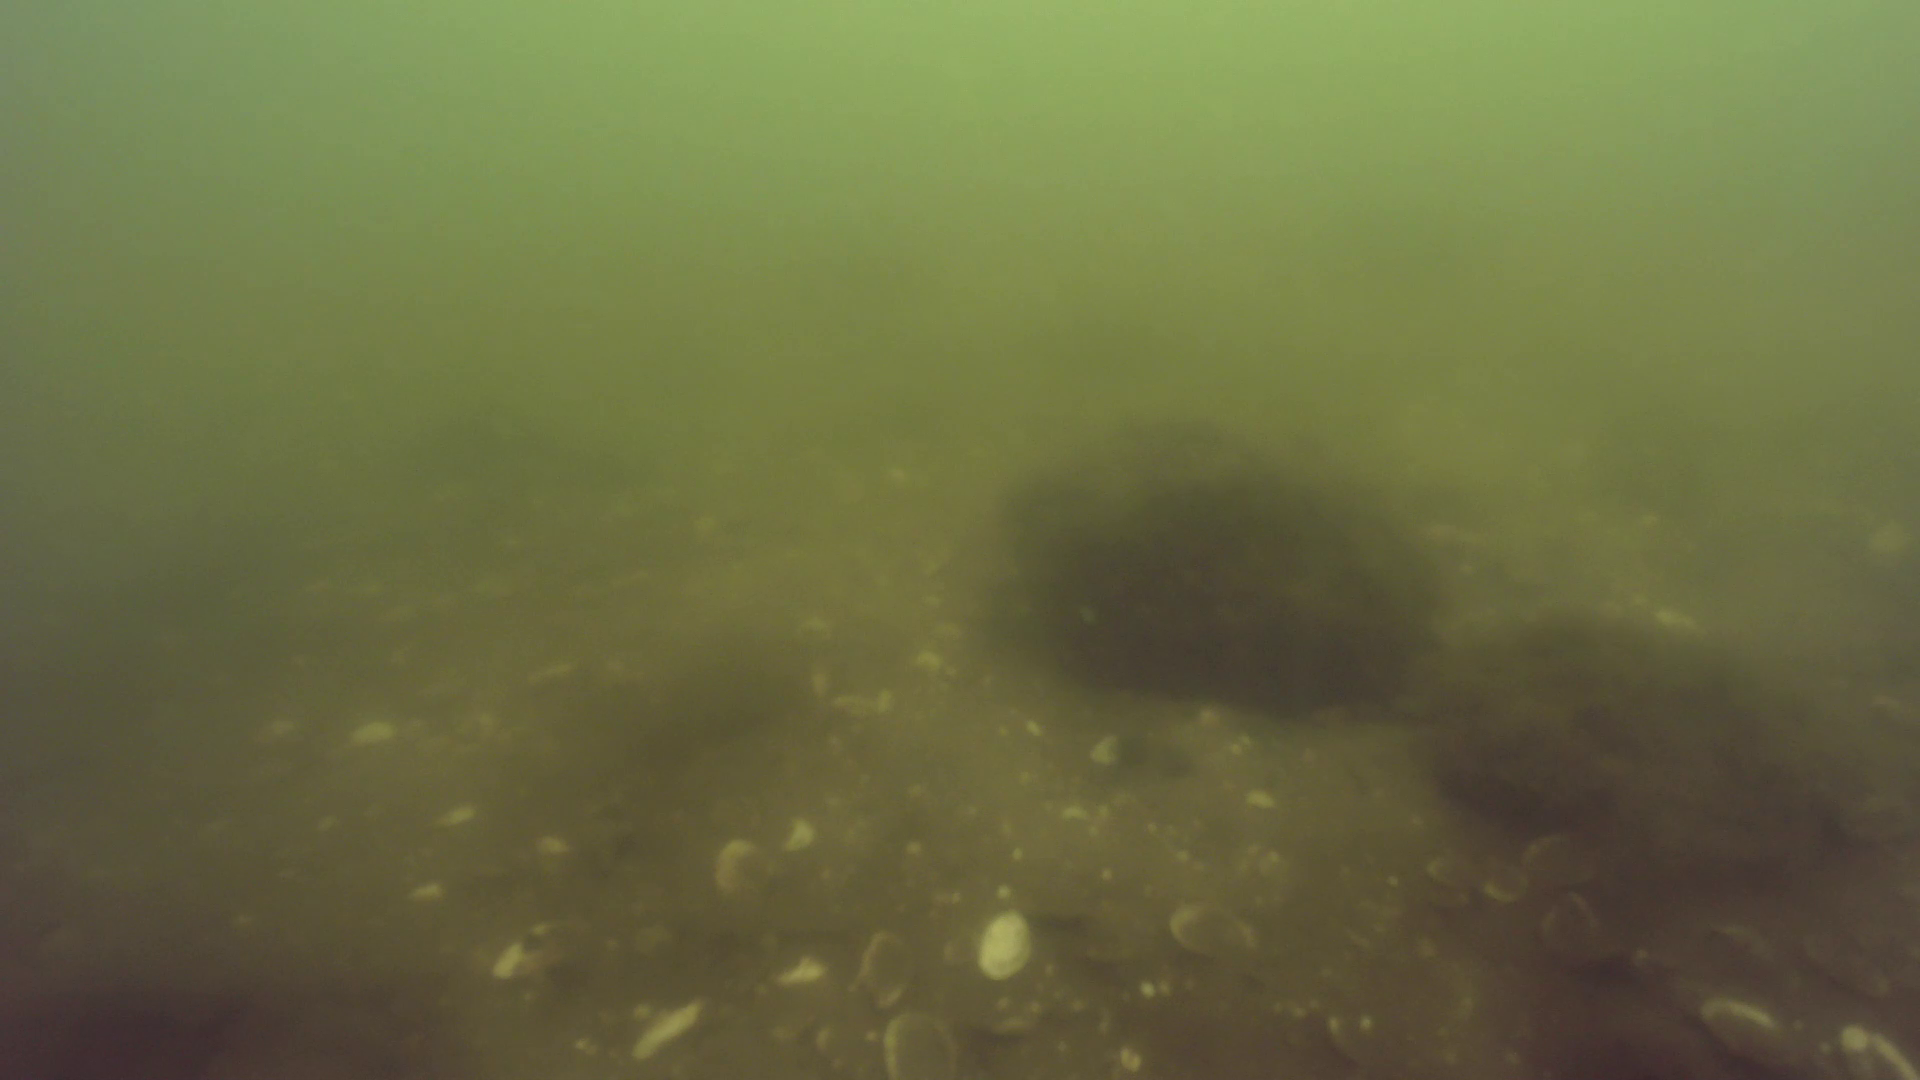
\includegraphics[height=\textheight,%
                   width=\textwidth,%
                   keepaspectratio]{Bilder/ROV/Steine.png}
\caption{Schlechte Unterwassersicht vor Lauerbach}
\end{figure}
\\

Insgesamt haben wir für unsere Forschung auf der Aldebaran an drei unterschiedlichen Stellen insgesamt fünf ROV Tauchgänge durchgeführt.
%Einfügen Karte mit Tauchstellen des ROV mit Objekten auf dem Multibeam
\subsubsection{Schwierigkeiten}
Während dieser Tauchgänge und bei deren Vorbereitung hatten wir einige unerwartete Schwierigkeiten.\\
Da die Aldebaran ein verhältnismäßig kleines Schiff für ein Forschungsschiff ist, hat sie zwar den Vorteil dass sie gerade durch das einklappbares Schwert einen sehr geringen Tiefgang von 80 cm hat, was uns die Forschung in diesem Gebiet erst ermöglicht hat.
Andererseits ist sie deshalb auch anfällig gegenüber Wind und Wetter, auch deshalb war das Arbeiten an Deck bei den zeitweise aufgetretenen Windstärken von vier bis fünf nicht immer einfach.\\
Dies hat sich sowohl bei der Vorbereitung des ROVs gezeigt als auch bei den Tauchgängen. Ein Problem war beispielsweise das Schwojen des Bootes am Anker.
Die Navigation und die Orientierung unter Wasser mit dem ROV war mit Abstand die größte Herausforderung, da die einzige Möglichkeit sich zu orientieren der eingebauter Kompass ist.
Unser ROV besitzt aufgrund seiner Größe kein USBL (Ultra Short Baseline) - System, wodurch die genaue Position des ROVs erst beim Auftauchen bekannt wird.
Eine durch das Multibeam angezeigte genaue Position haben wir angetaucht, indem wir diese über die Position des Schiffes angepeilt und versucht haben, bei Anfahrt durch den ROV diesen auf dem exakten Kompasskurs zu halten.
Durch das o.g. Schwojen ist die Fehlerquote hierbei schnell größer als die Sichtweite in der Ostsee. \\ Zusätzlich wurde das ROV 
durch die geringe Tauchtiefe von ca. 5m von den Wellendynamik und windinduzierter Strömung erfasst und im Kurs beeinflusst. 
Da wir selbst das ROV bisher lediglich auf Binnengewässern operiert haben, mussten wir zwangsläufig in vitro Erfahrungen mit dem ROV im Meereseinsatz sammeln, was die Trefferquote beim Anfahren interessanter Punkte zugegebenermaßen weiter verschlechterte. So spielte eine gute Portion Glück mit herein, was das Finden des angepeilten Objektes anging.\\
Trotz der Schwierigkeiten haben wir einige interessante Objekte mithilfe der optischen Kamera untersuchen können.\\



\section{Ergebnisse}
\section{Diskussion der Ergebnisse}

% Activate the following line by filling in the right side. If for example the name of the root file is Main.tex, write
% "...root = Main.tex" if the chapter file is in the same directory, and "...root = ../Main.tex" if the chapter is in a subdirectory.
 
%!TEX root = TNTinderSee.tex 

\chapter[Fazit]{Fazit}





% Activate the following line by filling in the right side. If for example the name of the root file is Main.tex, write
% "...root = Main.tex" if the chapter file is in the same directory, and "...root = ../Main.tex" if the chapter is in a subdirectory.
 
%!TEX root =  TNTinderSee.tex

\chapter[Danksagungen]{Danksagungen}
Wir danken Prof Dr. Jens Greinert vom GEOMAR Kiel und Leiter der Arbeitsgruppe DeepSea-Monitoring. Er ist einfach der beste Wissenschaftspate, den wir uns hätten wünschen können.\\


Frank Schweikert und Dr. Hannes Imhof von der deutschen Meeresstiftung, für die tollen Tage und all die Hilfe an Board der Aldebaran. \\


Mareike Kampmeier vom GEOMAR Kiel für die geduldige Einführung am Multibeam und die vielen Erklärungen zum Thema Sprengstoffe im Wasser. \\


Dr. rer. nat. Inken Suck vom GEOMAR Kiel, der bestimmt coolsten ROV-Piloten dafür, dass sie uns gezeigt hat, wie man Unterwasserfahrzeuge richtig navigiert. \\


Maria Martinez Cabanas vom GEOMAR Kiel dafür, dass sie uns und unsere Proben in Ihre Labore mitgenommen hat, und geduldig stundenlang alle Fragen beantwortet hat.\\



Yifan Song vom GEOMAR Kiel dafür, dass er uns ganz praktisch beigebracht hat, wie man Videomaterial georeferenziert.

Besonders beeindruckt hat uns, dass uns die Wissenschaftler:innen wie selbstverständlich Samstag und Sonntag zur Seite standen und uns alles gezeigt haben.

Vielen Dank auch an Svenja Ehlers vom GEOMAR für ihre Hilfe und Geduld was das administrative der Reise anging und natürlich auch an Sofie Steinhausen von der deutschen Meeresstiftung, für die stets hilfsbereite Begleitung während des ganzen Wettbewerbes.


Dr. Kevin Köser vom GEOMAR Kiel für den inspirierenden Vortrag über Photogrammetrie \\


Yifan Song vom GEOMAR Kiel dafür, dass er uns ganz praktisch beigebracht hat, wie man Videomaterial georeferenziert.\\

Marek Czernohous für die insgesamt über 24 Stunden Fahrzeit, die Mate, Franzbrötchen und enorme Hilfe beim \LaTeX -Satz.\\



\bibliography{bibliography}
\bibliographystyle{plain}
% Activate the following line by filling in the right side. If for example the name of the root file is Main.tex, write
% "...root = Main.tex" if the chapter file is in the same directory, and "...root = ../Main.tex" if the chapter is in a subdirectory.
 
%!TEX root =  TNTinderSee.tex

\chapter[Anhang]{Anhang}




\end{document}